\section[تمرین دوم - سؤال چهارم: انتخاب ویژگی افزایشی Forward Selection]
{\faProjectDiagram\ \ تمرین دوم ـ سؤال چهارم: پیاده‌سازی انتخاب ویژگی افزایشی (\lr{Forward Selection}) بر روی سرطان سینه}

\begin{stepbox}

\field{هدف و معرفی مسئله}{
هدف این بخش، بررسی مسئله **انتخاب ویژگی (\lr{Feature Selection})** به روش **افزایشی (\lr{Sequential Forward Selection - SFS})** بر روی مجموعه داده سرطان سینه (\lr{cancer.csv}) است.

هدف اصلی انتخاب ویژگی، کاهش ابعاد مسئله، حذف ویژگی‌های تکراری و نویز، جلوگیری از بیش‌برازش (\lr{Overfitting}) و افزایش تفسیرپذیری مدل با حفظ حداکثر دقت دسته‌بندی می‌باشد.
}

\field{بررسی اولیه داده‌ها و پاکسازی داده‌های پرت}{
مجموعه داده اولیه شامل $569$ نمونه، یک ستون شناسه (\lr{id})، ستون هدف \lr{diagnosis} (با برچسب‌های \lr{M} بدخیم و \lr{B} خوش‌خیم) و $30$ ویژگی پزشکی عددی است.

به منظور پالایش داده‌ها، با استفاده از روش محدوده بین‌چارکی ($\text{IQR}$)، نمونه‌های دارای مقادیر پرت شناسایی و حذف گردیدند. در نهایت $398$ نمونه پاکسازی‌شده برای مرحله آموزش و ارزیابی باقی ماندند.
}

\field{پیاده‌سازی طبقه‌بند و انتخاب ویژگی افزایشی (SFS)}{
از مدل **رگرسیون لوجستیک (\lr{Logistic Regression})** به عنوان طبقه‌بند پایه استفاده شد. روند اجرا به شرح زیر است:

\begin{enumerate}
\item **مدل کامل (با ۳۰ ویژگی):** ابتدا مدل با تمامی $30$ ویژگی آموزش داده شد که به دقت آموزش $95.6\%$ و دقت آزمون $95.0\%$ دست یافت.
\item **اعمال SFS:** با استفاده از ماژول \lr{\texttt{SequentialFeatureSelector}} از کتابخانه \lr{Scikit-Learn}، تعداد ۵ ویژگی برتر به صورت مرحله به مرحله انتخاب شدند.
\end{enumerate}

ویژگی‌های منتخب عبارتند از:
\begin{itemize}
\item \lr{\texttt{texture\_mean}} (میانگین بافت)
\item \lr{\texttt{smoothness\_mean}} (میانگین همواری)
\item \lr{\texttt{perimeter\_se}} (خطای معیار محیط)
\item \lr{\texttt{texture\_worst}} (بدترین بافت)
\item \lr{\texttt{area\_worst}} (بدترین مساحت)
\end{itemize}
}

\field{ارزیابی و مقایسه با ماتریس آشفتگی}{
ماتریس‌های آشفتگی (\lr{Confusion Matrix}) برای دو حالت کامل ($30$ ویژگی) و منتخب ($5$ ویژگی \lr{SFS}) در تصویر زیر رسم شده‌اند:

\vspace{0.4cm}

\begin{center}
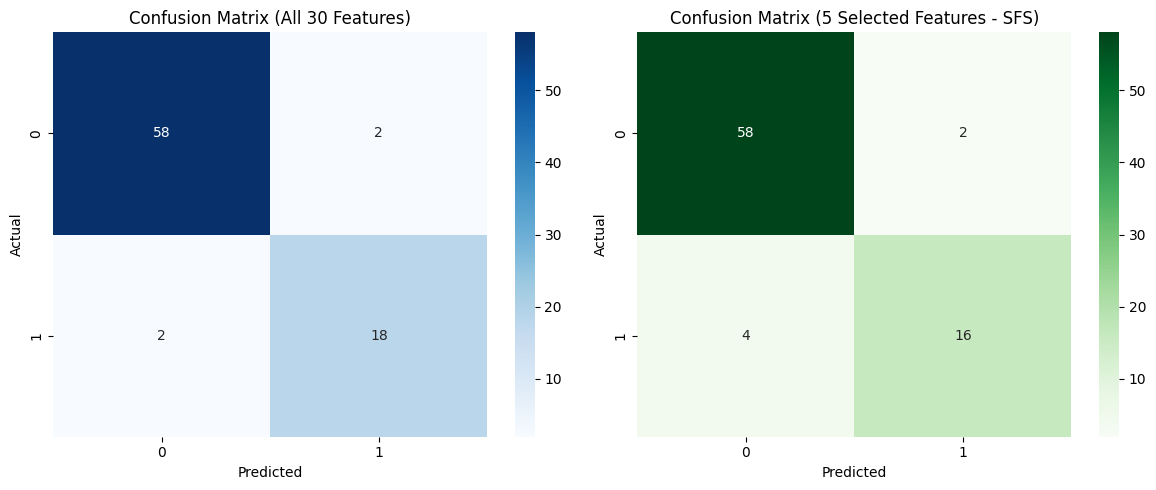
\includegraphics[width=.90\textwidth]{images/confusion_matrices.png}
\captionof{figure}{مقایسه ماتریس آشفتگی مدل با کل ۳۰ ویژگی (سمت چپ) و ۵ ویژگی منتخب \lr{SFS} (سمت راست)}
\label{fig:sfs_cm}
\end{center}

\begin{itemize}
\item **تحلیل ماتریس کامل (۳۰ ویژگی):** از ۸۰ داده آزمون، ۵۸ نمونه منفی واقعی (\lr{True Negative}) و ۱۸ نمونه مثبت واقعی (\lr{True Positive}) به درستی پیش‌بینی شده‌اند و تنها ۴ خطای مجموع وجود دارد (دقت $95\%$).
\item **تحلیل ماتریس SFS (۵ ویژگی):** با تنها ۵ ویژگی، تعداد ۵۸ منفی واقعی و ۱۶ مثبت واقعی به درستی تشخیص داده شده‌اند (دقت $92.5\%$).
\item **توجیه علت انتخاب این ویژگی‌ها:** الگوریتم \lr{SFS} ویژگی‌هایی را انتخاب کرده است که اطلاعات غیرتکراری ارائه می‌دهند؛ ترکیب شاخص‌های بافت (\lr{texture}) و اندازه خطیر غده (\lr{area\_worst} و \lr{perimeter\_se}) بیشترین قدرت تفکیک بافت‌های بدخیم و خوش‌خیم را فراهم ساخته است.
\end{itemize}
}

\field{جمع‌بندی}{
نتایج نشان داد که با کاهش $83\%$ ابعاد ویژگی‌ها (از ۳۰ به ۵ ویژگی)، دقت مدل تنها $2.5\%$ افت داشته است که نشان‌دهنده کارایی بالای الگوریتم \lr{Forward Selection} در بهینه‌سازی مدل‌های پزشکی می‌باشد.
}

\end{stepbox}